\chapter{Lecture 35 - Non-homogeneous Problem in Spherical Coordinates}
\label{ch:lec35}
\section{Objectives}
\begin{itemize}
\item Solve the time-dependent heat equation in spherical coordinates.
\item Provide another example illustrating how non-homogeneous boundary conditions can be treated.
\item Show another MATLAB solution.
\end{itemize}
\setcounter{lstannotation}{0}

\section{Non-homogeneous Heat Equation on a Sphere}

Consider the time-dependent temperature within a unit sphere as described by the following boundary value problem:

\begin{table}[h]
\begin{tabular}{l l}
$\substack{\text{Governing} \\\text{Equation}}: $& $\frac{\partial u}{\partial t} = \frac{\partial^2 u}{\partial r^2} + \frac{2}{r}\frac{\partial u}{\partial r}, \ \ 0<r<1, \ \ t>0$ \\
& \\
$\substack{\text{Boundary} \\ \text{Conditions}}: $& $u(1,t)=100, \ \ t>0$\\
& \\
$\substack{\text{Initial} \\ \text{Conditions}}: $ & $u(x,0) = 0, \ \ 0<r<1 $ \\
\end{tabular}
\end{table} 

Notice that we have omitted portions of the Laplacian, in spherical coordinates, containing derivatives of $\phi$ and $\theta$.  This is owing to the boundary conditions and initial conditions that are constants along with uniform material properties.\sidenote{We have omitted the thermal diffusivity, so you should assume $\alpha^2 = 1$.}  Thus we have considerably simplified the equation.  Having said that you should also notice that the boundary condition at $r=1$ is non-homogeneous.  We will not be able to solve this problem using separation of variables without dealing with that boundary condition first.

\newthought{Readers may recall} from Lecture 27 that we were able to deal with (some types of) non-homogeneous terms in the governing equation and boundary conditions by assuming a solution of the form: $u(x,t) = v(x,t) + \psi(x)$.  The boundary value problem that we derived for $\psi(x)$ absorbed all of the non-homogeneous terms leaving a homogeneous boundary value problem for $v(x,t)$ that we could solve using separation of variables.  We will pursue a similar strategy in this lecture. What we will do is:

\begin{enumerate}
\item Verify that---$\frac{\partial^2 u}{\partial r^2} + \frac{2}{r}\frac{\partial u}{\partial r}$---from the governing equation, can be expressed as: $\frac{1}{r}\frac{\partial^2}{\partial r^2}(ru)$.  This is easily verified:
\begin{align*}
\frac{1}{r}\frac{\partial^2}{\partial r^2}(ru) &= \frac{1}{r}\frac{\partial}{\partial r}\left[\frac{\partial}{\partial r}(ru)\right] \\
&= \frac{1}{r}\frac{\partial}{\partial r}\left[u + ru_r\right] \\
&= \frac{1}{r}\left[u_r + u_r + ru_{rr}\right] \\
&= u_{rr} + \frac{2}{r}u_r
\end{align*}

and

\item Let $ru(r,t) = v(r,t) + \psi(r)$ where $\psi(r)$ will once again be used to absorb the nonhomogenaities.  In this case we will also need to take care to only use solutions $\frac{1}{r}v(r,t)+\frac{1}{r}\psi(r)$ that remain bounded as $r \to 0$.
\end{enumerate}

\newthought{Let us now} restate the boundary value problem in terms of $ru(r,t)=v(r,t)+\psi(r)$. The governing equation becomes:
\begin{align*}
\frac{1}{r}\frac{\partial^2}{\partial r^2}\left[v(r,t) + \psi(r)\right] &= \frac{\partial}{\partial t}\left[\frac{1}{r}v(r,t) + \frac{1}{r}\psi(r)\right] \\
\frac{1}{r}\left[v_{rr} + \psi_{rr}\right] &= \frac{1}{r}v_t
\end{align*}
The boundary condition becomes:
\begin{align*}
u(1,t) &= 100 \\
\frac{1}{1}v(1,t) + \frac{1}{1}\psi(1) &= 100 \\
v(1,t) + \psi(1) &= 100
\end{align*}\marginnote[-1.5cm]{The boundary condition in the new form is $\frac{1}{r}v(r,t)\Big|_{r=1} + \frac{1}{r}\psi(r)\Big|_{r=1}$} And the initial condition is:
\begin{align*}
u(r,0) &= 0 \\
\frac{1}{r}v(r,0) + \frac{1}{r}\psi(r) &= 0
\end{align*}
We will take the boundary value problem for $\psi(r)$ therefore to be:
\begin{align*}
\frac{1}{r}\psi_{rr} &= 0 \\
\Rightarrow \psi_{rr}&= 0 \\
\psi(1) &= 100
\end{align*}

\vspace{2.0cm}

\noindent and the boundary value problem for $v(r,t)$ to be:
\begin{table}[h]
\begin{tabular}{l l}
$\substack{\text{Governing} \\\text{Equation}}: $& $v_{rr} = v_t, \ \ 0<r<1, \ \ t>0$ \\
& \\
$\substack{\text{Boundary} \\ \text{Conditions}}: $& $v(1,t)=0, \ \ t>0$\\
& \\
$\substack{\text{Initial} \\ \text{Conditions}}: $ & $v(r,0) = -\psi(r), \ \ 0<r<1 $ \\
\end{tabular}
\end{table} 

\vspace{0.25cm}

\newthought{Let us first} solve for $\psi(r)$:
\begin{align*}
\psi(r) &= 0 \\
\psi(1) &= 100
\end{align*}
The general solution is $\psi(r) = c_1r + c_2$.  Applying the boundary condition we get: $\psi(1) = c_1(1) + c_2 = 100$. There are infinitely many values for $c_1$ and $c_2$ that could satisfy this condition but we need to remember that $\frac{1}{r}\psi(r)$ must remain bounded as $r \to 0$.  This we will choose to set $c_2 = 0$ and $c_1 = 100$ so that:
\begin{equation}
\psi(r) = 100r
\label{eq:lec35-psi-sol}
\end{equation}

\newthought{Now we will turn} to the solution of the boundary value problem for $v(r,t)$ using separation of variables.

\vspace{0.25cm}

\noindent\textbf{Step \#1:} Assume a product solution.
\begin{equation*}
v(r,t) = F(r)G(t)
\end{equation*}

\vspace{0.25cm}

\noindent\textbf{Step \#2:} Insert the product solution into the governing equation.
\begin{align*}
\frac{\partial^2}{\partial r^2}\left[F(r)G(t)\right] &= \frac{\partial}{\partial t}\left[F(r)G(t)\right] \\
F_{rr}G &= FG_t
\end{align*}


\vspace{0.25cm}

\noindent\textbf{Step \#3:} Separate variables.

\begin{align*}
\frac{F_{rr}G}{FG} &= \frac{FG_t}{FG} \\
\frac{F_{rr}}{F} &= \frac{G_t}{G} = -\lambda
\end{align*}
So the separated equations are:
\begin{align*}
F_{rr} + \lambda F&= 0 \\
G_{t} + \lambda G &= 0
\end{align*}

\vspace{0.25cm}

\noindent\textbf{Step \#4:} Apply boundary conditions to determine non-trivial product solution(s).

\vspace{0.25cm}

\noindent For this problem, our boundary conditions are that $v(1,t) = 0$ and that $\frac{1}{r}v(r,t)$ should remain finite as $r \to 0$.  Rather than go through the analysis exhaustively, for this lecture we will claim that $\lambda > 0$ and set $\lambda = \alpha^2, \ \alpha>0$. This means that:\marginnote{Interested readers should show that for $\lambda < 0$ or $\lambda = 0$ there are no no-trivial solutions that will both satisfy the boundary condition and not diverge as $r \to 0$.}
\begin{align*}
F(r) &= c_3\cos{\alpha r} + c_4\sin{\alpha r} \\
G(t) &= c_5e^{-\alpha^2 t}
\end{align*}
In order to satisfy the requirement as $r \to 0$, we will set $c_3 = 0$ since $\frac{1}{r}\cos{\alpha r}$ diverges as $r \to 0$.  As for the rest of $F(r)$:
\begin{align*}
F(1) = c_4\sin{\alpha} &= 0 \\
\Rightarrow \sin{\alpha} &= 0 \\
\Rightarrow \alpha &= n \pi, \ \ n=1,2,3,\dots
\end{align*}
So the product solution is:

\begin{equation}
v(r,t) = \sum\limits_{n=1}^{\infty} c_n \sin{(\alpha_n r)}e^{-\alpha^2 t}
\label{eq:lec35-ex-sol-v}
\end{equation}

\vspace{0.25cm}

\noindent\textbf{Step \#5:} Satisfy the initial condition.
\begin{align*}
v(r,0) = \sum\limits_{n=1}^{\infty}c_n \sin{(\alpha_n r)}(1) &= -\psi(r) \\
\sum\limits_{n=1}^{\infty} \sin{(\alpha_n r)} &= -100r 
\end{align*}
On the left we have an infinite linear combination of eigenfunctions, on the right we have a function.  We need to determine the values of the constants $c_n$ so that the two are equal.  How do we do this?  We will multiply both sides by an orthogonal function and integrate.  The result is:
\begin{equation}
c_n = \frac{\int_{0}^1 -100r \sin{(\alpha_n r)} \ dr}{\int_0^1 \sin{(\alpha_n r)}^2 \ dr}
\label{eq:lec35-v-coeff}
\end{equation}

\newthought{The last step} will be to combine the solutions for $\psi(r)$ and $v(r,t)$ to form $u(r,t)$:
\begin{align*}
ru(r,t) &= v(r,t) + \psi(r) \\
u(r,t) &= \frac{1}{r}\left[ v(r,t) + \psi(r)\right] \\
u(r,t) &= \underbrace{\frac{1}{r}\sum\limits_{n=1}^{\infty}c_n \sin{(\alpha_n r)}e^{-\alpha_n^2 t}}_{\text{transient}} \underbrace{+ 100}_{\substack{\text{steady}\\ \text{state}}} 
\end{align*}
where the formula for the coefficients is given in Equation \ref{eq:lec35-v-coeff}.\marginnote[-1.5cm]{As in Lecture 27, we find that $v(x,t)$ corresponds to the transient solution, and $\psi(r)$ is the steady-state solution.}

\section{MATLAB Implementation}

The code to construct this solution is straight-forward and presented in its entirety in the listing below.

\begin{lstlisting}[name=lec35-ex, style=myMatlab]
clear
clc
close 'all'

%% Parameters
N = 50;

c = 1; % radius of sphere
Psi = @(r) 100.*r;
R = @(r,n) sin(n.*pi.*r);
T = @(t,n) exp(-((n.*pi).^2).*t);

V = @(r,t) 0; % initialize my approximation for V

for n = 1:N
   % compute coefficient
   cn = 2*integral(@(r) -Psi(r).*R(n,r),0,c);
   
   % update solution to V
   V = @(r,t) V(r,t) + cn.*R(r,n).*T(t,n);
end

% construct solution U
U = @(r,t) (1./r).*(V(r,t)+Psi(r));
\end{lstlisting}
Plots of the solution at various time, $t$, are presented below.

\begin{figure}[h!]
\subfloat[]{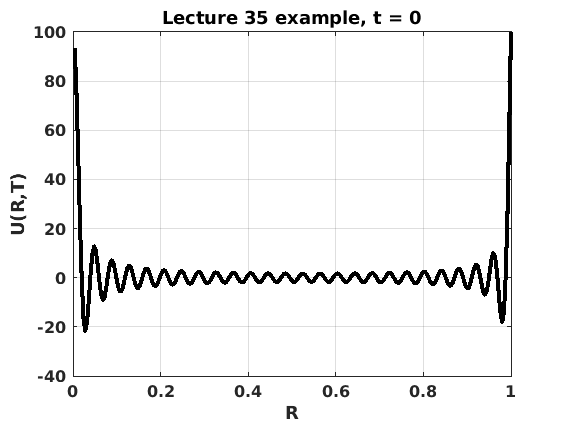
\includegraphics[width=2in]{lec35-t0.png}}
\subfloat[]{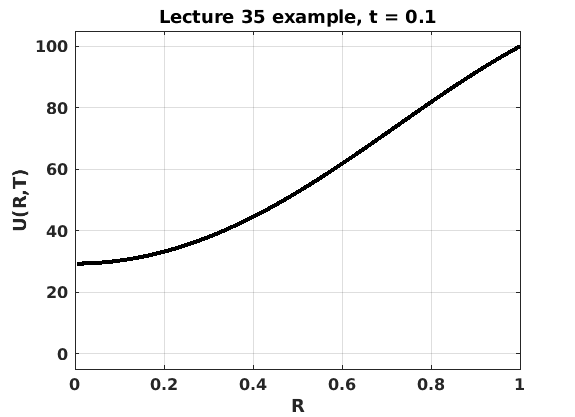
\includegraphics[width=2in]{lec35-t0p1.png}} \\
\subfloat[]{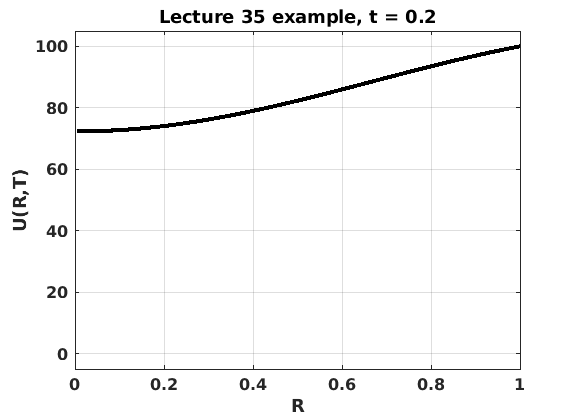
\includegraphics[width=2in]{lec35-t0p2.png}}
\subfloat[]{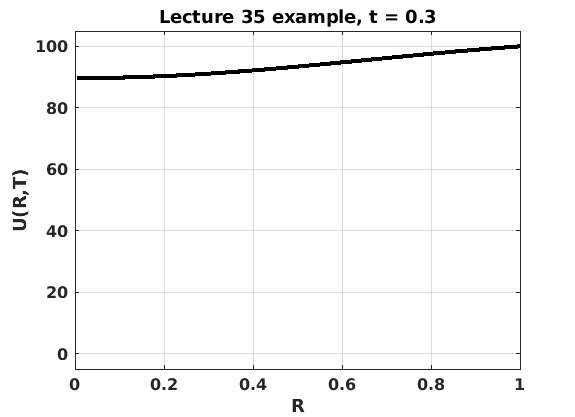
\includegraphics[width=2in]{lec35-t0p3.png}} \\
\subfloat[]{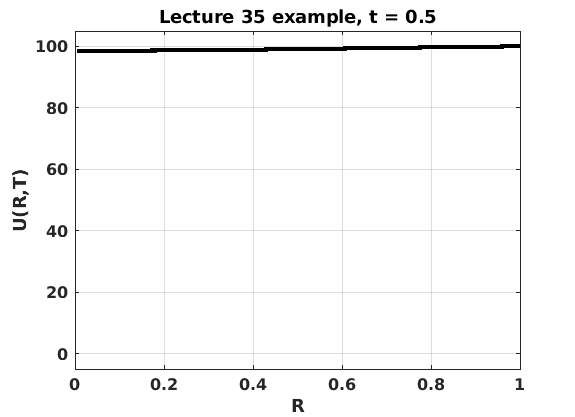
\includegraphics[width=2in]{lec35-t0p5.png}}
\subfloat[]{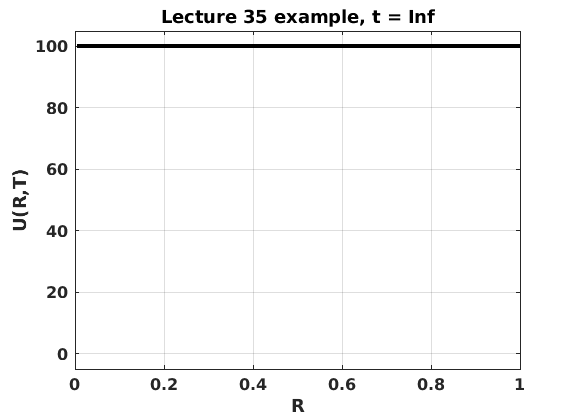
\includegraphics[width=2in]{lec35-tinf.png}}
\label{fig:lec35-ex-plots}
\caption{Plots solution at various times.}
\end{figure}

